
\chapter{Assoziative Arrays}
\section{Datenstrukturdreieck am Beispiel Assoziativer Arrays}
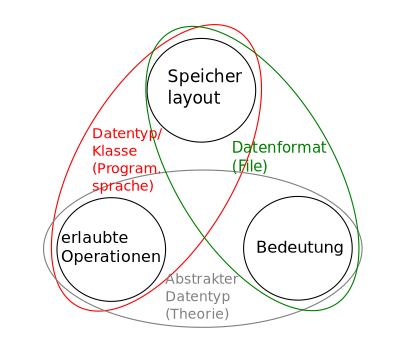
\includegraphics[width=16cm,height=8cm,keepaspectratio]{./Pictures/Datenstrukturdreieck.png}\\
\begin{tabular}{L{4cm} | L{5cm} | L{5.5cm}}
     \multicolumn{1}{c}{\textbf{Abstrakter Datentyp}} & \multicolumn{1}{c|}{} & \textbf{Datentyp in Python} \\ \hline
    Operationen & Bedeutung & Welche Fkt. implementiert man? \\ \hline
    Schlüssel k , Werte v, Array a &  & Hilfsklasse Node \\ \hline
    \verb|a[k] = v| & Speichere v unter dem Schlüssel k oder ersetze Daten, falls k vorhanden & \verb|__setitem__(self, k, v)| \\ \hline
    \verb|v = a[k]| & frage Daten vom Schlüssel k ab, Fehlermeldung falls k nicht vorhanden & \verb|__getitem__(self, k)| \\ \hline
    \verb| a.has_key(k)| & True, wenn k vorhanden & \verb| has_key(self, k| \\ \hline
    \verb|del a[k]| & Lösche Schlüssel k und seine Daten, oder Fehlermeldung, wenn k nicht vorhanden & \verb|__delitem__(self, k)| \\ \hline
    \verb|len(a)| & aktuelle Anzahl der Schlüssel bzw. Schlüssel/Wert-Paare & \verb|__len__(self)| \\ \hline
\end{tabular}\\

k im Prinzip beliebig (Anforderungen später) \\

Fileformate für assoziative Arrays:
\begin{itemize}
    \item lesbar für Menschen und Maschinen (als Textfiles): XML, JSON, YAML
    \item nur lesbar für Maschinen (als Binärfile): HDF5
\end{itemize}

\section{JSON-Format}
\subsection*{7.2.1 Spezifikation des JSON-Formats}
in Backus-Naur-Notation: \\
\begin{tabular}{L{2cm} C{1cm} L{10cm}}
    JSON-file & := & array $|$ \\
    & $|$ & dictionary \\
    array & := & '[' \hspace*{5mm} elements \hspace*{5mm} ']'\\
    & $|$ & '[' \hspace*{1cm} ']'  \hspace*{1cm} \#leeres Array\\
    elements & := & value \\
    & $|$ & value ',' elements \\
    dictionary & := & '\{' \hspace*{5mm} pairs \hspace*{5mm} '\}' \\
    & $|$ & '\{' \hspace*{1cm} '\}'\hspace*{1cm} \#leeres Dictionary \\
    pairs & := & \textcolor{red}{string} ':' value \\
    & $|$ & \textcolor{red}{string} ':' value ',' pairs \\
    string & := & '\grqq' \hspace*{5mm} '\grqq'\hspace*{1.3cm} \#leerer String\\
    & $|$ & '\grqq' characters '\grqq' \\
    value & := & \textcolor{blue}{number} $|$ \textcolor{blue}{string} $|$ \textcolor{blue}{boolean} $|$ \textcolor{blue}{null} $|$ array $|$ dictionary\\
\end{tabular}\\

\textcolor{red}{Schlüssel} \\
\textcolor{blue}{werden als Zeichen im UTF-8 Zeichensatz codiert}

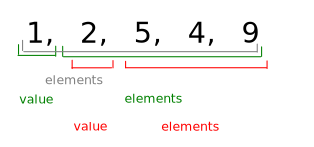
\includegraphics[width=16cm,height=2cm,keepaspectratio]{./Pictures/komischesArray.png}

\subsubsection*{Beispiel für JSON: Studenten-Datenbank}
\begin{minted}{python}
Students = {
    "Fritz Mueller": {
        "Mathematik": [2.0, 1.7, 1.3],
        "ALDA":       1.3
    },
    "Anna Weise": {
        "Mathematik":  [1.0, 1.0, 1.0];
        "Philosophie": 1.3
    }
}
\end{minted}
Einlesen von JSON in Python: json-Modul

\begin{minted}{python}
import json
students = json.load(file("students.json").read().decode("utf_8"))
\end{minted}

\vspace*{1cm}

\begin{tabular}{L{8.5cm} | L{7cm}}
    \textbf{Anforderungen an die Schlüssel :} & Implementation \\ \hline
    \verb|key1 == key2| & sequentielle Suche $\bigO{}(N)$ \\ \hline
    Ordnung \verb|key1 < key2| (impliziert \verb|key1 == key2|) & binäre Suchbäume, binäre Suche $\bigO{}(log N)$ \\ \hline
    \verb|key1 == key2| & Hashtabelle \hspace*{2cm} $\bigO{}(1)$ \\
    \verb|hash(key1) => integer| & \\
\end{tabular}

\vspace*{1cm}

